\chapter{Understanding the effect of IAC on looking up information}

\begin{mynote}
\subsubsection{Chapter outline}
The previous chapter demonstrated that for an expenses task, people have to copy data from multiple sources that differ in terms of their IAC. This chapter describes two studies that explore the extent to which IACs influence strategies, speed and accuracy. 

Study 3 tests how IAC affects switching behaviour when copying from one source. It tested whether the effect of IAC on copying colours, as shown in previous studies, extends to copying numbers. Study 4 tests how IAC affects switching behaviour when information for one entry task has to be collected from multiple sources.
Together these studies intend to show that IAC affects how people switch between entering and looking up information.

\end{mynote}

 
\section{Study 3: Copying numbers from one source}\label{ch:Study2}
\subsection{Introduction}
Study 1 and 2 illustrated that people had to retrieve and copy data from multiple sources with varying information access costs (IAC). People were not always able to look at the data source while entering data, and information sometimes had to be briefly kept in memory before people could enter it.
In this situation, people have various options: they can decide to keep going back to the target source, reduce their memory load by writing it down, or keep as much of it in memory. Participants in Study 1 explained they tried to do it in the quickest way possible, and preferred to keep data in memory as this was often a faster strategy than writing it down, printing it out, or going back and forth between the source and the input window.

This is in line with previous lab studies, which showed that as the cost to access information increases, people increasingly rely on the information in their head rather than the information in the environment \citep[e.g.][]{Gray2006, Morgan2009}. People look at the target source longer before copying anything, but after one look, they do enter more items in one sequence before looking back. 

\citet{Gray2004} conducted a study where people had to copy over VCR programming information. Participants either had permanent access to the information, the information was covered by a grey box which could be uncovered by hovering over it with the cursor, or they were explicitly instructed and trained before the trial to memorise the information. The people in the latter condition were more accurate than the other conditions in entering the information. This shows that a deeper encoding of the information in memory makes people more accurate in entering the information. 

In later studies that further explored the effect of access costs on use of memory, the Blocks World Task (BWT) was used as a task paradigm, which requires people to copy a 3x3 grid of coloured blocks. In these studies, participants relied more on memory as the cost to access the target window increased. In one study, this memory-based strategy made participants better able to resume after interruptions by copying more blocks before having to revisit the target window \citep{Morgan2009}. Looking at overall task performance overall however, they did make more errors overall and took considerably longer to complete the task. In a later paper, the researchers reflected that the coloured blocks participants had to copy may have been too demanding to memorise \citep{Waldron2011}. This abstract visuo-spatial information did not bear any meaning to the participant, in contrast with the VCR programming information used in \citet{Gray2004} which is more familiar and easy to memorise. This suggests that the type of information to copy influences the effect that IAC might have on task performance, though the studies differed in task paradigm making it hard to compare their findings: in \citet{Gray2004} people were explicitly instructed to memorise the information and conducted a test prior to a trial during which they had to fill in the information, and could not continue until they had stated everything correctly. This ensured that people had the information well-memorised before they started the experimental trial. In the Blocks World Task studies, participants were not given this training or instruction.

Rather than training participants to memorise the information, \citet{Soboczenski2013} used an alternative approach to motivate people to encode the information more deeply. They conducted two studies where people had to transcribe text and numbers that were presented either in a black font colour or a harder-to-read grey font colour. Participants made fewer data transcription errors if data was shown in the harder-to-read font colour, both for transcribing text and numbers. In line with \citet{Gray2004}, these studies showed that when people do make the effort to more deeply encode information in a copying task, it can improve their accuracy.

In order to design data entry interfaces that support how people enter expenses from information sources with varying IACs, it is important to understand how these differences in IAC affect strategy and task performance. Relying on information in the head over information in the world can make it more likely for people to make errors in a copying task\citep{Morgan2009}, though other studies have shown that a deeper encoding of information can also improve accuracy if memorised well \citep{Gray2004, Soboczenski2013}. 

The study reported in this chapter replicates the BWT study, by using both coloured and numbered blocks.The purpose of this study is to see whether the effect on IAC on people's strategies and performance, as reported in previous BWT studies, holds when people have to copy numbers instead of colours.

It is expected that the effect of IAC on strategy will be similar and that an increase in IAC will encourage people to adopt a more memory-based strategy.  However, the expectation is that numbers are easier to memorise and people will be able to memorise more items. Furthermore, based on previous findings that a deeper encoding of numbers in memory can reduce errors, it is expected that an increased IAC will improve accuracy for copying numbers.


\subsection{Method}
\subsubsection{Participants}
Fourty-two participants (eight male) were recruited from the UCL Psychology Subject Pool. Ages ranged from 18 to 52 with a mean age of 22.38 (SD = 7.45). Participants received course credit or \pounds3.75 as a compensation for taking part in the study.

\subsubsection{Design}
A mixed design was used with two independent variables: IAC and block type.
The between-participants variable was the level of IAC which had three levels. If the IAC was Low, the target pattern was permanently visible. In the Medium and High IAC conditions, the target pattern was covered with a grey mask, and could only be uncovered by moving the mouse cursor over the window. The mask reappeared as soon as the cursor left the window. In the High IAC condition, there was an additional 1-second delay to uncover the mask. This delay time was used in previous BWT studies where it showed to have a significant effect on task strategies and performance \citep{Gray2006, Morgan2009, Waldron2007}.
The within-participants variable was the block type to be copied, which was either coloured or numbered blocks. The order was counter-balanced across participants.

The dependent variables are listed in Table \ref{table:ch4_dvs}. The primary focus is on the measures of the first visit, as participants do not have any information yet on the target pattern. On subsequent visits, they may already have partial information in their head from previous visits. Therefore, the items copied after the first visit is believed to be the most 'sensitive measure of performance' \citep{Janssen2012}. 
Two dependent variables were used to measure accuracy. Incorrectly placed blocks measured instances where a participant initially placed a block in the incorrect place, but then moved this to the correct place prior to submitting the pattern. Incorrectly submitted trials measured instances where the participant had finished copying a pattern and clicked the Submit button, but the pattern was incorrect.

\begin{table}[htp]
\centering
    \begin{tabular}{  l }
    \hline
    \textbf{ Strategy measures} \\  
    Number of visits to target window  \\ 
    Visit duration of first visit (s)  \\
    Average duration of visits (s) \\
    Number of blocks copied after first visit \\
    Number of blocks copied correctly after first visit 
    
    \vspace{10pt} \\
    
\textbf{Global task performance measures} \\ 
Number of incorrectly placed blocks (per trial) \\
Number of incorrectly submitted trials (per experiment block) \\
Trial completion time incl. and excl. lockout (s) \\ \hline
    \end{tabular}
    \caption[Study 3 dependent variables]{Dependent variables used in the study.}
    \label{table:ch4_dvs}
\end{table}

\subsubsection{Materials}
\begin{figure}[]
\begin{center}

\begin{subfigure}[b]{\textwidth}
\centerline{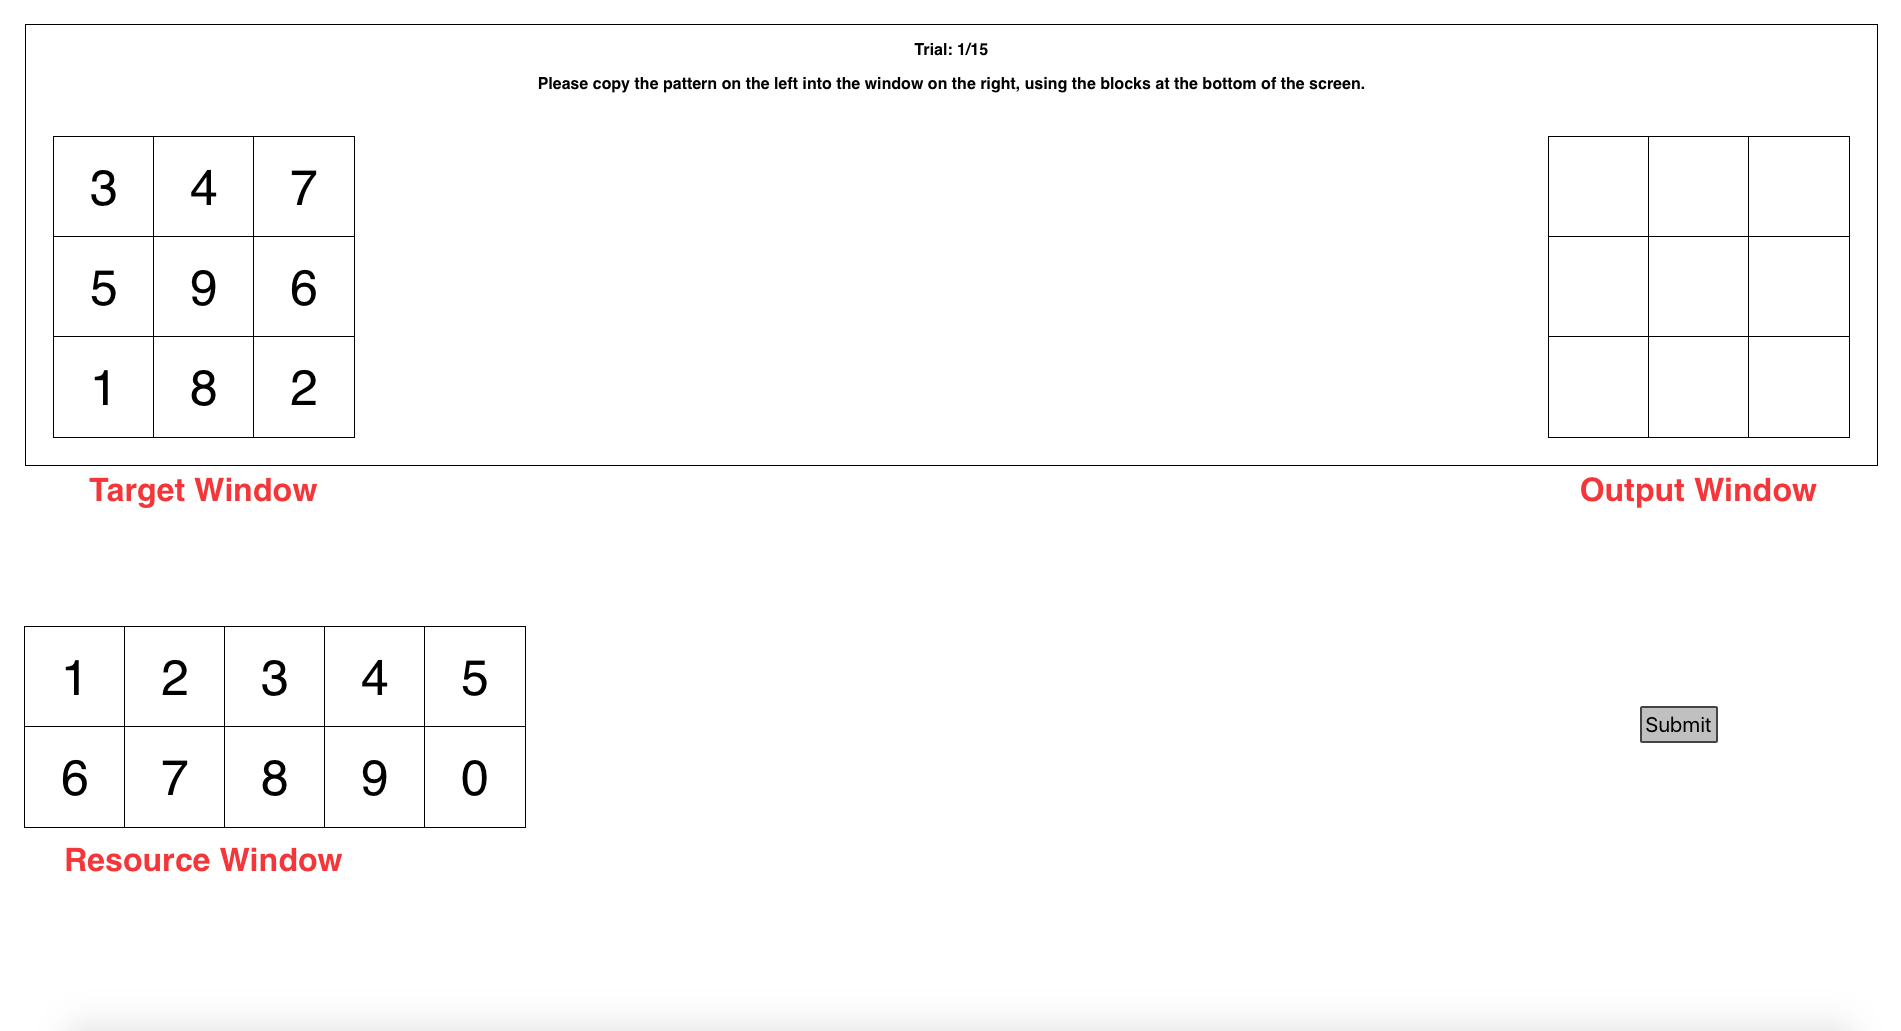
\includegraphics[scale=0.23]{images/Study2/ch4_numbers.png}}
\caption{The number condition.}
\label{fig:ch4_BWT}
\end{subfigure}
%\hfill%
\begin{subfigure}[b]{0.5\textwidth}
\centerline{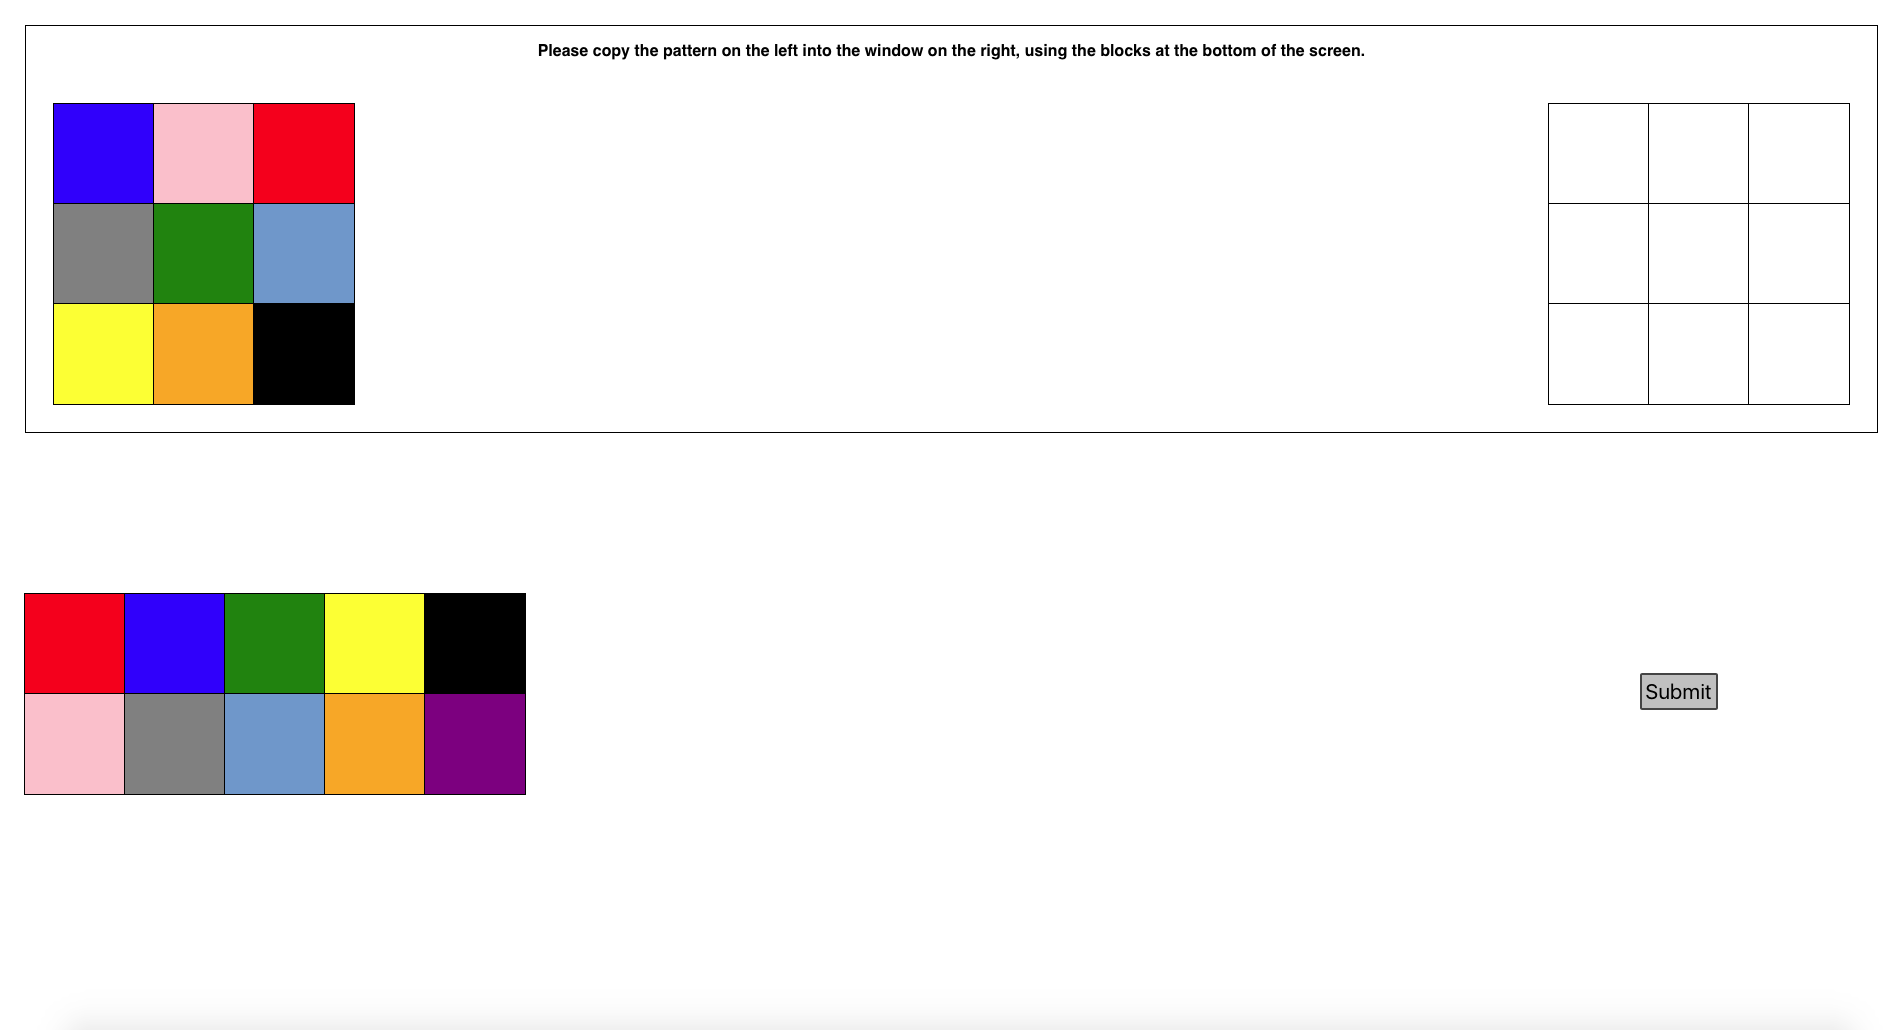
\includegraphics[scale=0.23]{images/Study2/ch4_colours.png}}
\caption{The colour condition.}
\label{fig:ch4_NWT}
\end{subfigure}
\caption[Study 3 task lay-out]{The task lay-out with the three different components.}
\label{fig:ch4_taskparadigm}
\end{center}
\end{figure}

Figure \ref{fig:ch4_taskparadigm} shows the task paradigm that was used. Each colour or number was only used once. The colours used were similar to the colours used in previous BWT studies \citep[e.g.][]{Gray2006, Morgan2009}.
Participants had to copy and complete fifteen patterns of each block type, and each participant had to copy over the same patterns. The target window showed a 3x3 grid with either coloured or numbered blocks. The output window showed an empty 3x3 grid, and was the same size as the target window. Participants had to copy the pattern shown in the target window by dragging blocks from the resource window and moving them into the output window. 

%Apparatus
The study was conducted on a desktop computer, using a 24-inch monitor with a resolution of 2048 x 1152 pixels. Participants used a computer mouse to drag and drop blocks. The experimental task was implemented using HTML, Javascript and PHP and run in a browser.  All relevant browser events, such as mouse movements to (un)cover the grey mask, dragging and dropping the blocks and mouse clicks, were recorded and saved in a mySQL database. The browser window covered the whole screen to minimise distractions.

For the Low IAC condition, eye fixations were used to measure the number and duration of visits to the target window. Eyetracking data was also obtained for the Medium and High IAC conditions. However, this data was not used due to the fact that people were able to also view the target window area whilst the target pattern was covered. Therefore, in accordance with previous IAC studies \citep[e.g.][]{Gray2004}, for the Medium and High IAC conditions the number and duration of uncovering the mask was taken as a measurement for visits to the target window.  These uncoverings were measured by Javascript. The usefulness and limitations of using these measures are discussed in the Discussion.

A Tobii T60 eyetracker was used for recording people's eye fixations. Eye movements were recorded at a rate of 60 gaze data points per second for each eye, with an accuracy of 0.5 degrees and timestamp accuracy of 4 ms. For the analysis, all consecutive eye fixations with no drag or drop actions in-between were added together and counted as one fixation.

\subsubsection{Procedure}
Participants were welcomed and briefed about the experiment. It was explained they would be shown nine blocks which were in a certain order, and had to copy this order by moving blocks around. Participants were instructed to complete the task as fast as possible, but it was explained that they were not able to continue until they had copied a pattern correctly. 
The experiment was broken down in two parts, one where they had to copy colours, and one where they had to copy numbers. For each part, they were given two practice trials first to get familiar with the set-up, and to give them a chance to ask questions if anything was unclear. There was an opportunity for the participant to take a break between the two parts. 
They were then asked to read and sign a consent form and given an information sheet with a summary of the study and the researcher's contact details. In addition to the verbal briefing, the explanation of the study was written out on the computer screen for the participant to read and they were shown an instruction video that showed how the experiment worked. The study took around 20-30 minutes to complete.

\subsubsection{Ethical considerations}\label{sec:quanethics}
The study was undertaken with ethical approval from the UCL Research Ethics Committee [Project ID Number UCLIC/1415/001/Staff Brumby/Borghouts]. 
At the start of each study, participants were first briefed verbally about the study. They were asked to read and sign a consent form, and were given an information sheet to keep. This information sheet contained a summary of the study information and the researchers' contact details. It was explained that an eyetracker would record their eye fixations and movements, but that these recordings were anonymous and that they would not be directly identifiable. After participants had completed the first part of the experiment, a prompt appeared on the screen advising them to take a short break. Participants could take a break as long as they wanted and could decide themselves when to continue with the second part of the experiment.

Participants were informed that the data would be used for research purposes only and stored in accordance with the Data Protection Act 1998. They were also informed that their data would be anonymised and when used in a report or academic paper, their data would not be directly identifiable. 
 
\subsection{Results}
The means and standard deviations of all dependent variables are shown in Table \ref{table:ch4_IACmeans}.

Eight participants were removed from the analysis due to weak eye-tracking calibration. Furthermore, one participant misunderstood the experiment and did not know she was allowed to uncover the mask of the target window more than once. This participant had scores that were more than three times the interquartile range from the rest of the participants' scores on six different variables, so this participant was considered an outlier and removed from the analysis. 


\begin{table*}\centering
\ra{1.3}
%\begin{tabular}{|p{6cm}|lll|lll|}\toprule
\begin{tabular}{@{}p{6cm}lllclll@{}}\toprule
%\begin{tabular}{  p{6cm} l p{1cm} l p{2cm} l  p{1cm}l p{1cm} | p{2cm} | p{1cm}|}
 & \multicolumn{3}{c}{\textbf{Colours}} & \multicolumn{3}{r}{\textbf{Numbers}} \\
 \cmidrule{2-4} \cmidrule{6-8}
 & Low & Medium & High && Low & Medium & High\\\midrule
\textbf{Strategy measures}\\
Number of visits to target window & \textbf{6.36} & \textbf{4.24} & \textbf{2.98} && \textbf{5.10} & \textbf{2.03} & \textbf{2.05} \\
						    & 		    2.28 & 		1.62   & 	          0.90 && 		2.48   & 	         0.63  & 	       0.67 \\
Visit time of first visit (s)  		    & \textbf{0.39} & \textbf{0.04} & \textbf{2.18} && \textbf{0.51} & \textbf{0.04} & \textbf{1.49} \\
				       		    &              0.23   & 		  0.02  & 	         1.59  && 		 0.45  & 	         0.05 & 	      1.01 \\
Average time of visits (s)  		    & \textbf{0.29} & \textbf{0.04} & \textbf{1.54} && \textbf{0.35} & \textbf{0.04} & \textbf{1.07} \\
				       		    &              0.13   & 		  0.02  & 	         0.95  && 		 0.15  & 	         0.03 & 	      0.77 \\
Number of blocks copied		    & \textbf{1.90} & \textbf{3.55} & \textbf{4.52} && \textbf{2.44} & \textbf{6.18} & \textbf{6.33} \\
 after first visit 		       		    &              1.84   & 		  1.93  & 	         1.43  && 		 1.89  & 	         1.61 & 	      1.67 \\
Number of blocks copied correctly & \textbf{1.86} & \textbf{3.22} & \textbf{4.07} && \textbf{2.36} & \textbf{5.96} & \textbf{5.98} \\
after first visit 		       		    &              1.75   & 		  1.83  & 	         1.20  && 		 1.74  & 	         1.52 & 	      1.55 \\

\vspace{10pt}

\textbf{Global task performance measures}\\
Number of incorrectly placed blocks 
				  		    & \textbf{0.15} & \textbf{0.67} & \textbf{0.79} && \textbf{0.17} & \textbf{0.31} & \textbf{0.46} \\
(per trial) 				       	    &              0.18   & 		  0.40  & 	         0.44  && 		 0.19  & 	         0.18 & 	      0.16 \\
Number of incorrectly submitted
				  		    & \textbf{0.27} & \textbf{1.9} & \textbf{2} && \textbf{0.36} & \textbf{0.5} & \textbf{0.83} \\
trials (per experiment block)	    &              0.65   & 		2.51 & 	   2.13  && 		 1.21  & 	         1.08 & 	      1.03 \\
Trial completion time incl. lockout
				  		    & \textbf{19.60} & \textbf{25.40} & \textbf{31.80} && \textbf{19.47} & \textbf{20.83} & \textbf{25.95} \\
(s)						    &                2.98   & 		5.16 & 	   	     6.08  && 	         3.03  & 	        3.08   & 	         4.21 \\
Trial completion time excl. lockout
				  		    & \textbf{19.60} & \textbf{25.40} & \textbf{28.84} && \textbf{19.47} & \textbf{20.83} & \textbf{23.89} \\
(s)						    &              2.98   & 		5.16 & 	   6.34  && 		 3.03  & 	         3.08 & 	      4.06 \\

\bottomrule
\end{tabular}
\caption[Study 3 descriptive measures]{The effect of IAC on copying colours and numbers. The means are shown in bold, the standard deviations are below the means.}
\label{table:ch4_IACmeans}
\end{table}

\subsubsection{Task strategies}

\subsubsection{Number of visits to the target window}
Participants made fewer visits to the target source when they had to copy numbers (M = 3.06, SD = 2.08) than when they had to copy colours (M = 4.49, SD = 2.18), F(1,30) = 41.62, p<.001, $\eta^2$  = 0.58. Participants also made fewer visits as IAC increased from Low (M = 5.73, SD = 2.41), to Med (M = 3.13, SD = 1.65), to High (M = 2.51, SD = 0.91), F(2,30) = 15.16, p<0.001, $\eta^2$  = 0.50. To investigate differences between conditions, post-hoc Tukey comparisons were performed. Results showed that participants made significantly fewer visits in the Medium-IAC condition than in the Low-IAC condition, p <.01. However, there was no difference in number of visits between the Medium-IAC and the High-IAC conditions, p=.59. Participants looked at the target window for colours more on every level of IAC (see Figure \ref{fig:ch4_noVisits}), and so there was no significant interaction, F(2,30) = 2.82, p=.08, $\eta^2$  = 0.16. 

\begin{figure}[!ht]
\centering
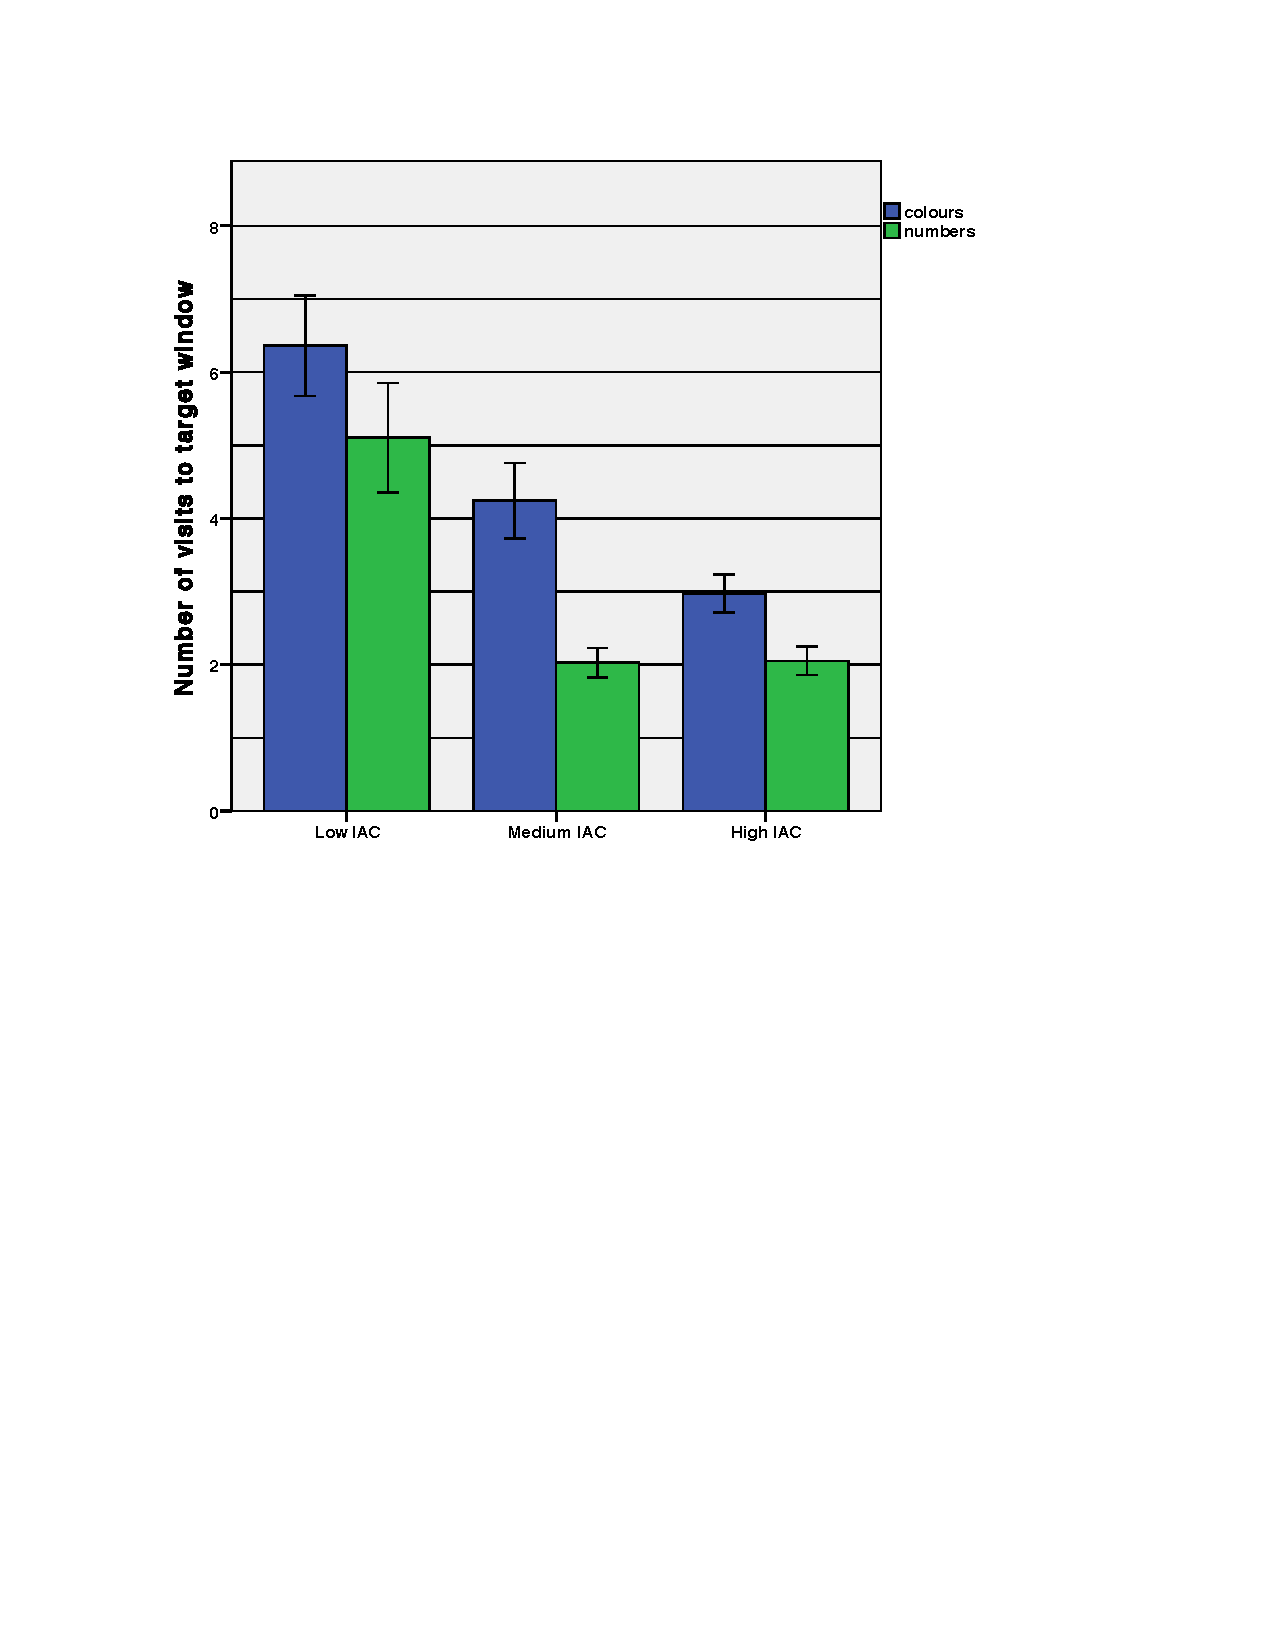
\includegraphics[width=\textwidth]{images/Study2/ch4_noVisits-bargraph.pdf}
\caption[Study 3 number of visits]{The interaction between block type and IAC for number of visits to the target window. The error bars represent $\pm $1 standard error.}
\vspace{-9pt}
\label{fig:ch4_noVisits}
\end{figure}

\subsubsection{Duration of first visit to target window}
There was no significant main effect of block type on the duration of the first visit, F(1,30) = 3.05, p=.09, $\eta^2$  = 0.09. Participants looked longer at the target source as IAC increased from Low to High. Post-hoc comparisons showed that participants looked longer in the High-IAC condition (M=1.84, SD = 1.35) than in the Low/Medium-IAC conditions, ps <.001. However, there was no difference in duration between the Low-IAC (M = 0.45, SD = 0.46) and the Medium-IAC (M = 0.05, SD = 0.04) conditions, p=.47. There was a significant interaction effect between IAC and block type, F(2,30) = 5.70, p<.01, $\eta^2$  = 0.28 (see Figure \ref{fig:ch4_firstVisitDuration}). There were no difference between block types in the Low-IAC condition, t(10) = -1.86, p = 0.09, nor the Medium-IAC condition, t(9) = -0.29, p = 0.7. However, in the High-IAC condition, participants looked significantly longer for colours (M = 2.18, SD = 1.59) than numbers (M = 1.49, SD = 1.01), t(11) = 2.76, p = 0.02.

\begin{figure}[!ht]
\centering
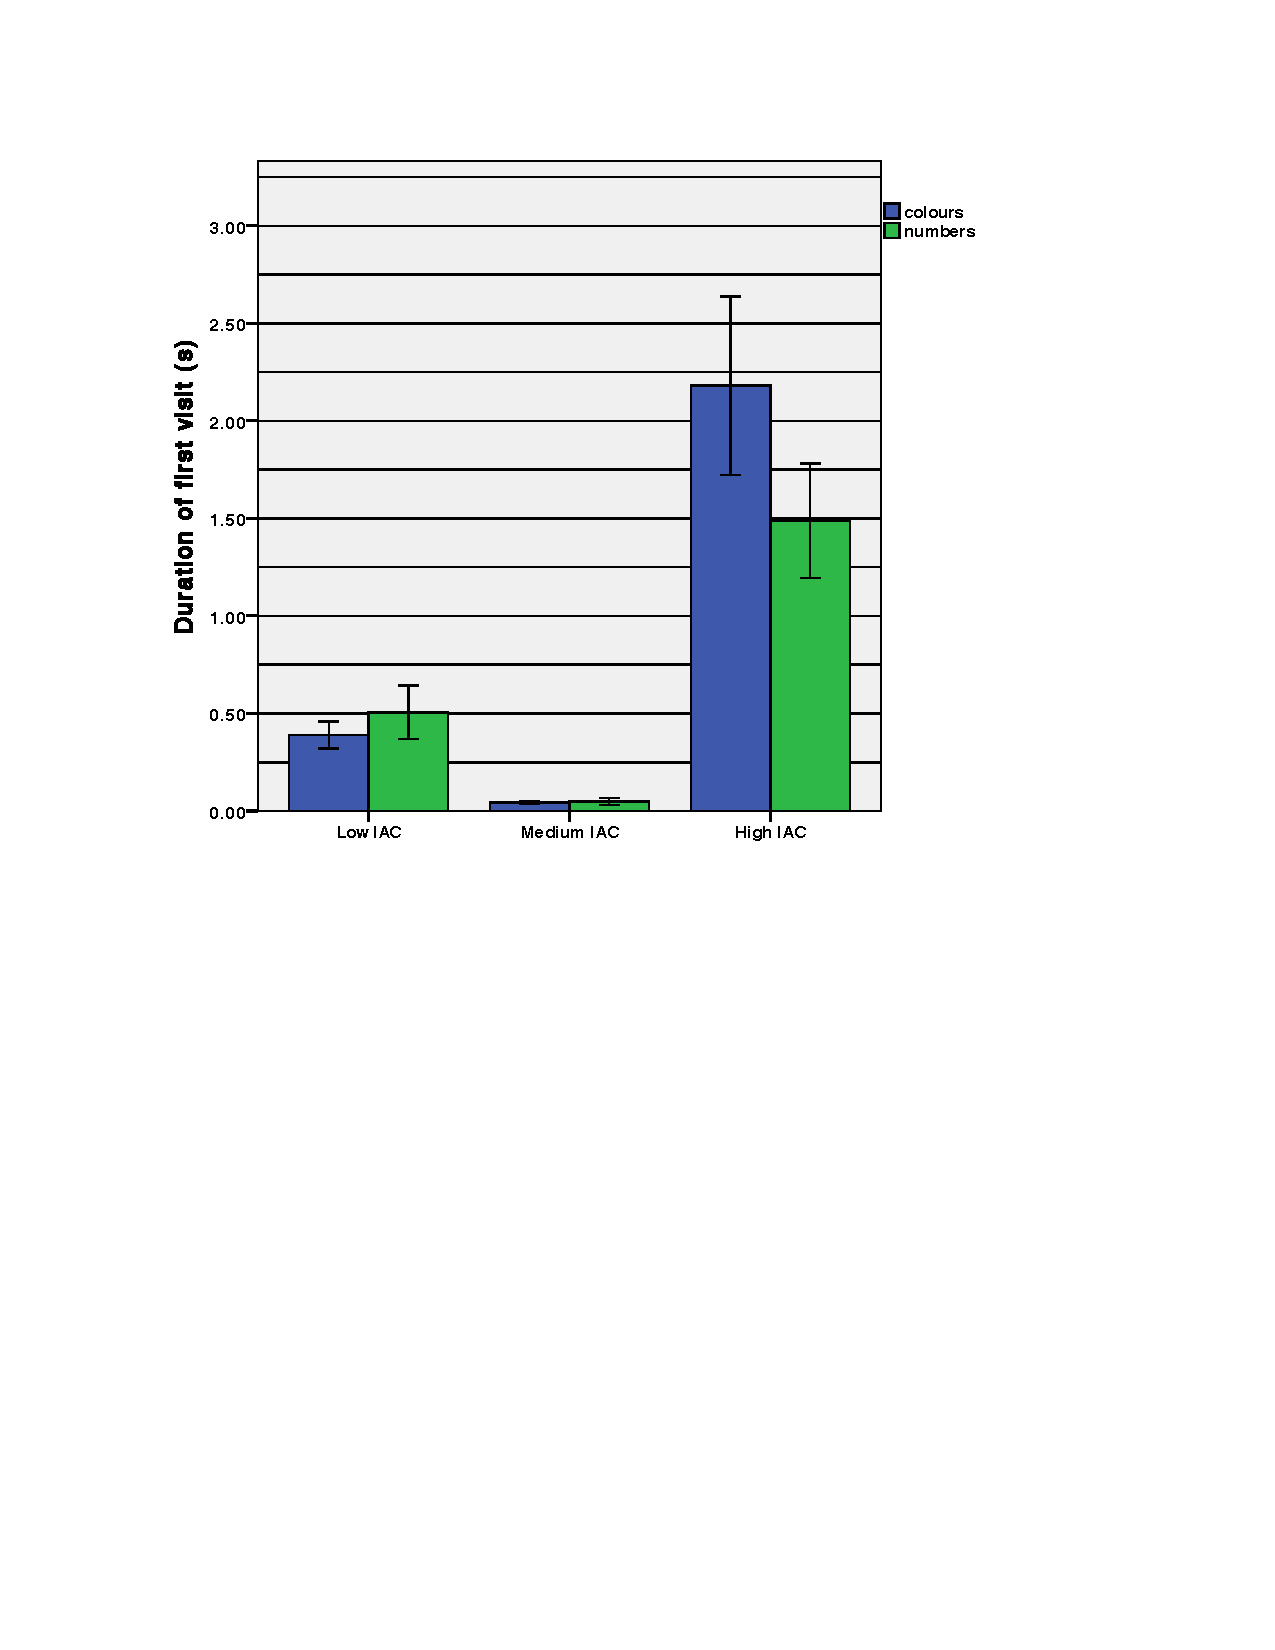
\includegraphics[width=\textwidth]{images/Study2/ch4_firstVisitDuration-bargraph.pdf}
\caption[Study 3 duration of first visit]{The effect of IAC on the duration of the first visit to the target window. The error bars represent $\pm $1 standard error.}
\vspace{-9pt}
\label{fig:ch4_firstVisitDuration}
\end{figure}

\subsubsection{Blocks placed after first visit}
People placed more blocks correctly after the first visit for numbers (M = 4.77, SD = 2.33) than colours (M = 3.08, SD = 1.81), F(1,30) = 63.86, p<.001, $\eta^2$  = 0.68. They also placed more blocks as IAC increased, F(2,30) = 12.54, p<0.001, $\eta^2$  = 0.46. Tukey post-hoc comparisons show there was a difference between the Low IAC and Medium/High IAC conditions (ps<.01), but not between Medium and High IAC conditions (p=.77). There was a significant interaction effect between IAC and block type, F(2,30) = 8.96, p<.01, $\eta^2$  = 0.37  (see Figure \ref{fig:ch4_firstCorrectBlocks}). When IAC was Low, the number of blocks that were copied correctly after the first visit did not differ significantly for colours or numbers.

\begin{figure}[!ht]
\centering
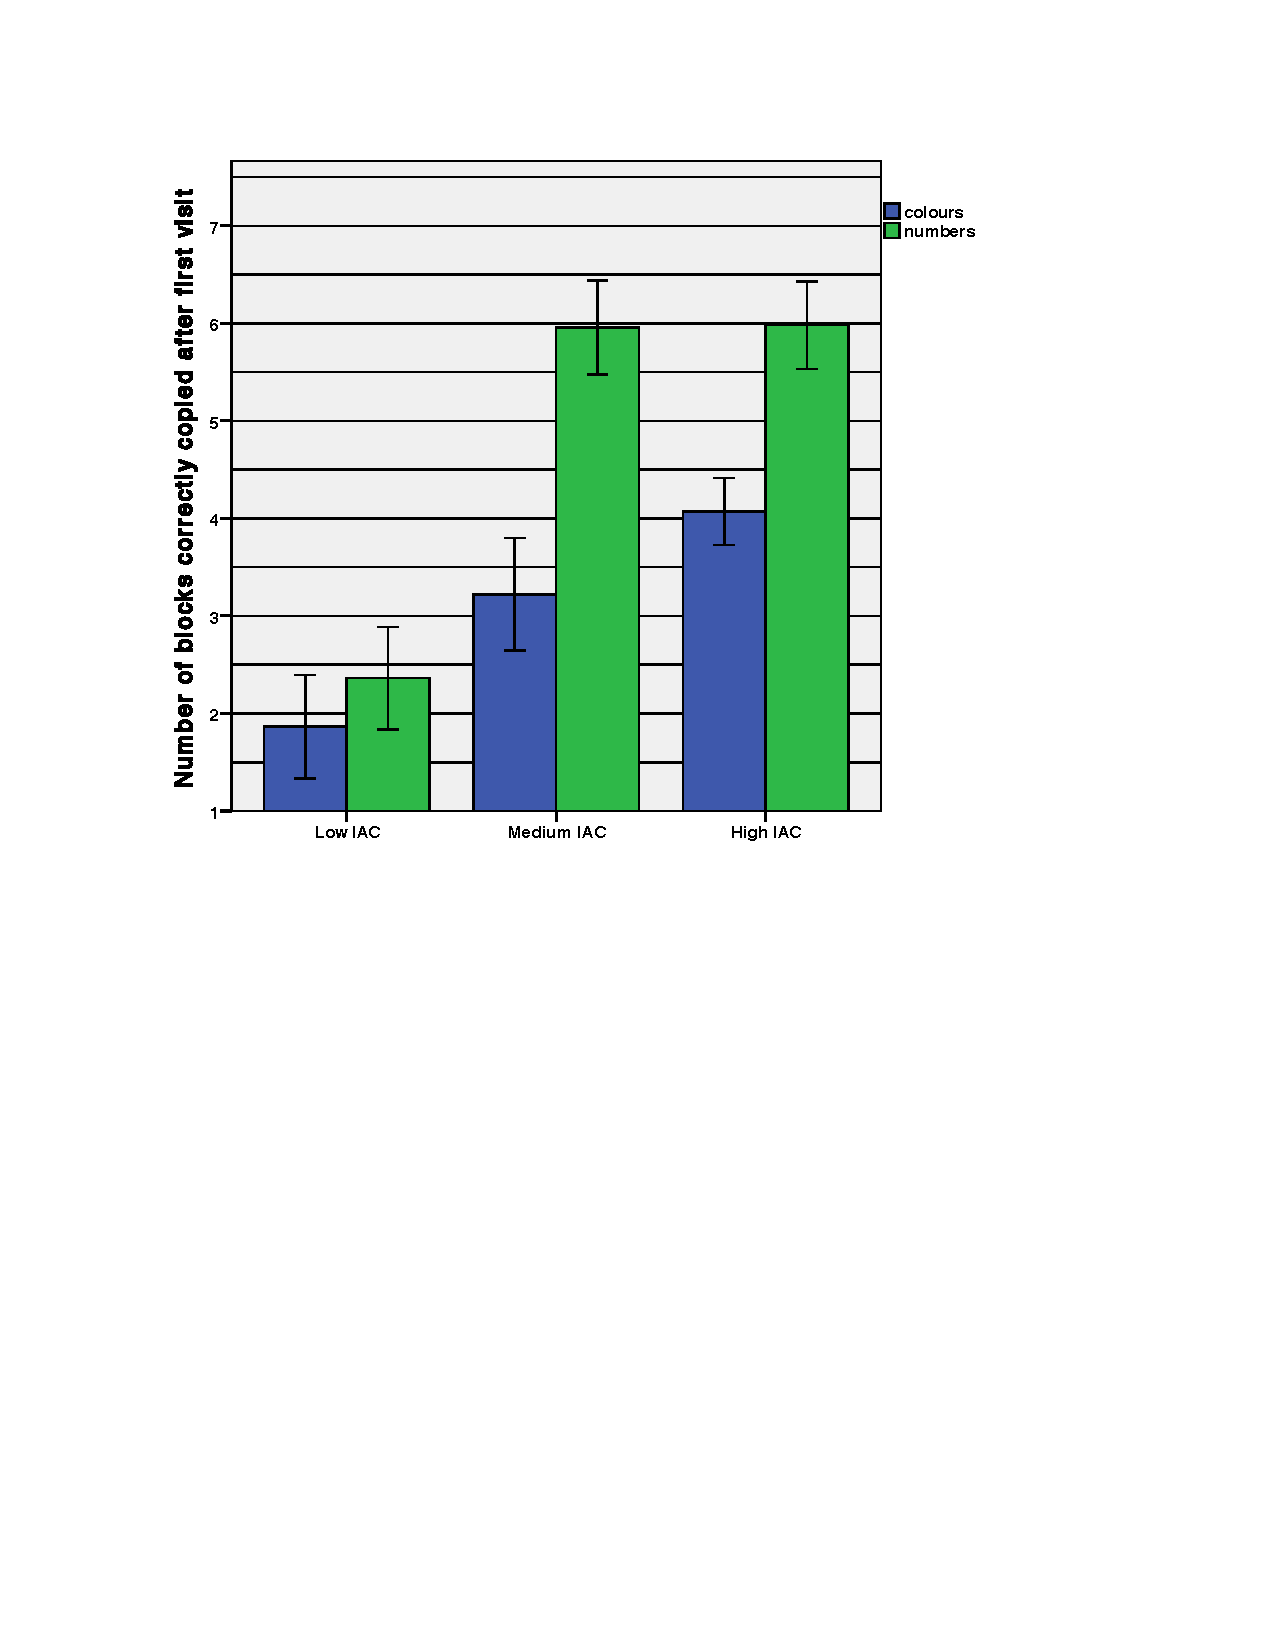
\includegraphics[width=\textwidth]{images/Study2/ch4_firstCorrectBlocks-bargraph.pdf}
\caption[Study 3 number of blocks correctly placed]{The interaction between block type and IAC for number of blocks correctly placed after the first visit to the target window. The error bars represent $\pm $1 standard error.}
\vspace{-9pt}
\label{fig:ch4_firstCorrectBlocks}
\end{figure}

\subsubsection{Global task performance}
The interactions between block type and IAC on global task performance measures all had the same trend: people performed the same for colours and numbers when IAC was Low, but differences appeared between the block types as IAC increased. As this trend was the same for each interaction, the statistical results of the interactions are reported but their specific trend will not be repeated.

\subsubsection{Number of incorrectly placed blocks}
Participants placed more blocks incorrectly for colours (M = 0.54, SD = 0.45) than numbers (M = 0.32, SD = 0.21), F(1,30) = 10.71, p=.003, $\eta^2$ = 0.26. As IAC increased and participants were keeping more items in memory, they increasingly placed more incorrect blocks, F(2,30) = 14.71, p<.001, $\eta^2$ = 0.50. Tukey post-hoc comparisons show there was a difference between the Low IAC condition (M = 0.16, SD = 0.18) and Medium/High IAC conditions (ps<.01), but not between the Medium (M = 0.49, SD = 0.35) and High IAC conditions (M = 0.63, SD = 0.36) (p = .3). There was a significant interaction effect between IAC and block type, F(2,30) = 3.36, p<.05, $\eta^2$ = 0.18. When IAC was Low, the number of blocks that were copied incorrectly did not differ significantly for colours or numbers, but as IAC increased, participants placed more blocks incorrectly for colours.

\subsubsection{Number of incorrectly submitted trials}
The number of trials that were submitted incorrectly was generally low, but participants submitted more incorrect trials for colours (M = 0.1, SD = 0.16) than numbers (M = 0.04, SD = 0.08), F(1,30) = 5.28, p=.029, $\eta^2$ = 0.15. There was no significant effect of IAC, F(2,30) = 2.70, p=0.08, $\eta^2$ = 0.15, nor any interaction, F(2,30) = 1.65, p=.2, $\eta^2$ = 0.10.

\subsubsection{Trial time}
Two trial completion times are considered here: total time and time excluding lockout. 
Looking at the actual completion time, participants took longer to complete a trial when they were copying colours (M = 25.80, SD = 7.06) compared to when copying numbers (M = 22.24, SD = 4.47), F(1,30) = 44.08, p<.001, $\eta^2$ = 0.60. As IAC increased from Low to Medium to High, participants took longer to complete a trial, IAC, F(2,30) = 15.91, p<0.001, $\eta^2$ = 0.52. Tukey post-hoc comparisons show there was a difference between Low/Medium and High (ps<.01), but not between Low and Medium (p = .12). There was a significant interaction effect between IAC and block type, F(2,30) = 11.05, p<.001, $\eta^2$ = 0.42. 

With the lockout time in the High-IAC condition removed, the same effects were found for block type, F(1,30) = 34.55, p<.001, $\eta^2$ = 0.54, and IAC, F(2,30) = 8.18, p=0.001, $\eta^2$ = 0.35. Tukey post-hoc comparisons show there was still a difference between Low and High (p=.001), but no longer between the Medium IAC and Low IAC or High IAC conditions (ps >.1). There was a significant interaction effect between IAC and block type, F(2,30) = 8.13, p=.002, $\eta^2$ = 0.35.

\subsubsection{Qualitative data}
The screen recordings from the eye-tracker were played back to further investigate people's behaviour. Although this helped understand some behaviour which could not be determined from the quantitative data alone, these observations only serve to explain some of the quantitative measures and are not the main focus of the analysis.

The visit durations in the Medium IAC condition were suspiciously short. Upon replaying the screen recordings, it appeared that participants often accidentally moved their cursor over the grey mask of the target source. This was counted as a visit by the program, even though participants may have not intentionally moved their cursor to this part of the screen to look at the target source. They did not spend a long time looking at the target window, but also did not immediately move blocks either, and sometimes waited multiple seconds before they made a move. 

\begin{figure}[!ht]
\centering
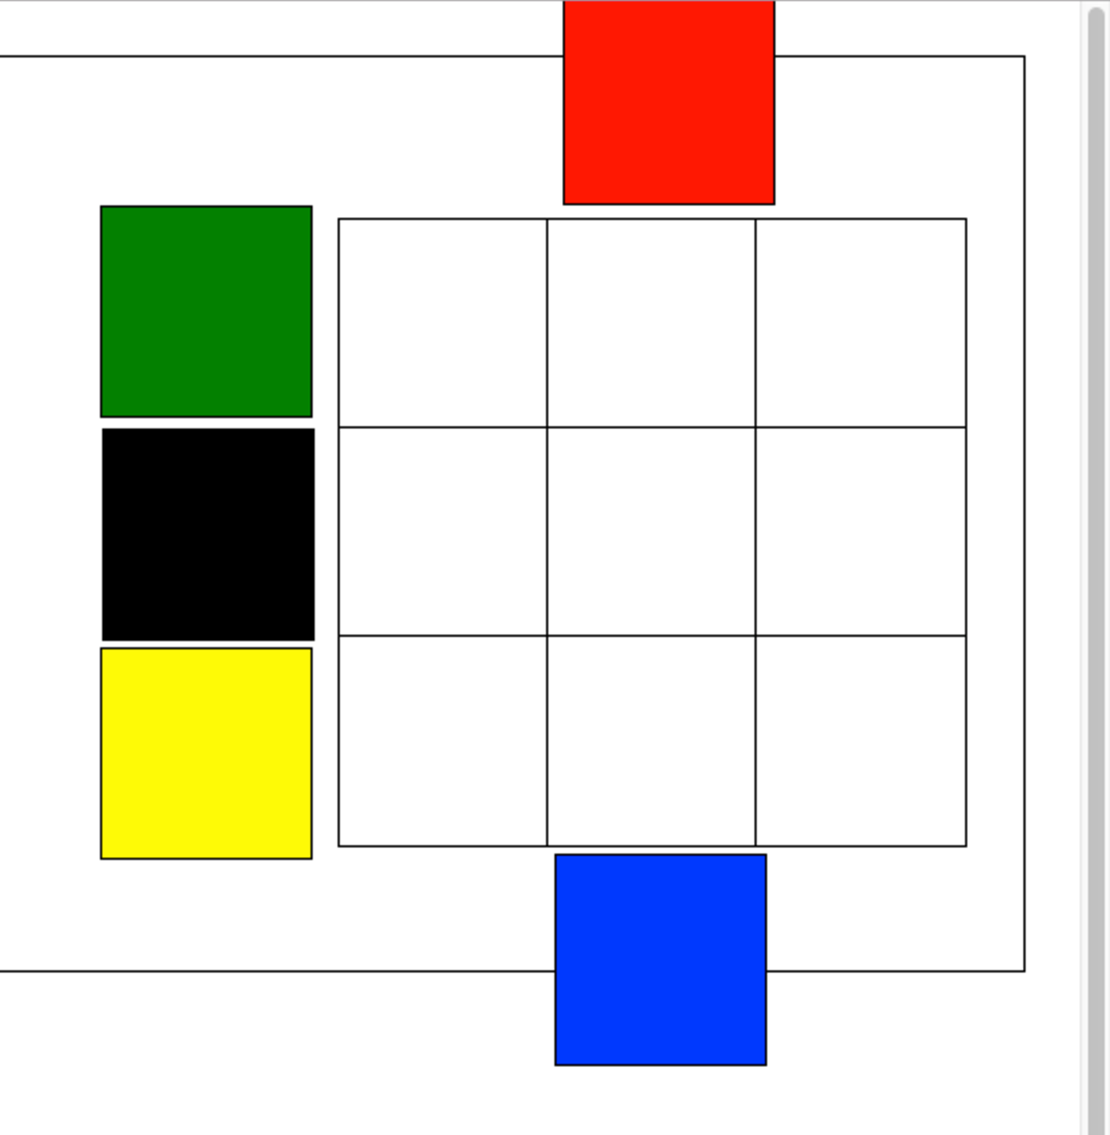
\includegraphics[scale=0.3]{images/Study2/ch4_placeholders.pdf}
\caption[Study 3 placeholders]{Participants placed blocks outside of the output window as `placeholders'.}
\vspace{-9pt}
\label{fig:ch4_placeholders}
\end{figure}

During the 1-s lockout in the High IAC condition, participants changed their minds about visiting the target window on numerous occasions. They placed their mouse cursor on the mask, but left this field before it was uncovered to move one or more blocks. It could be this decision also occurred in the Medium IAC condition, but as there was no lockout the mask was already uncovered before people made this decision, and would explain the very short visits.

People sometimes placed the blocks as `placeholders' as shown in Figure \ref{fig:ch4_placeholders}: they placed several blocks outside of the output window next to the position they thought it belonged to, but did not place it there yet. Only after viewing the target again, they placed the blocks in the output window. Looking at quantitative data alone, this type of strategy would be depicted as one long view at the target, after which all blocks were placed in one go. This is true to some extent, but as people could already place the blocks and offload their memory without this being recorded by the program, they only had to check if this position was correct on the subsequent visit, and is different from a strategy where people spent a long time trying to memorise the blocks after which all blocks were placed.


\newpage

\subsection{Discussion}
This study replicated the Blocks World Task with the aim to see if the effect on IAC on a copying task, as previously found when using colours, can be extended to copying numbers, and if a deeper encoding of numbers into memory makes people more accurate.

The main findings are:

\begin{itemize}
\item
Numbers are easier to copy than colours, but only if IAC is increased
\item
Increases in IAC make people adopt memory-intensive strategies
\item
Increases in IAC increases errors
\end{itemize}

\subsubsection{The effect of block type on task strategies and performance}
Changing the block type from colours to numbers made it easier to memorise the blocks: people made shorter and fewer visits than when copying colours, but were still able to place more blocks. This difference in performance is only found in the Medium and High IAC conditions, which further suggests the difference between numbers and colours is due to the memorability of the information, and the interactions on most of the dependent variables further show that the difference between block types was dependent on the level of IAC.

The difference between numbers and colours fit well with the distinction in Baddeley's \citeyearpar{Baddeley1986} seminal model of working memory between processing visuo-spatial and verbal information. As numbers can be rehearsed and therefore refreshed in working memory, they are likely easier to memorise. After the study had ended, several participants in this study explained they used some sort of rehearsal and tried to say the numbers out loud in their head. For colours, some indicated they tried to either capture a mental picture of the colours in their mind, while others rehearsed the word for each colour (e.g. 'red' and 'blue') but they felt they were able to remember fewer items using this strategy. This is consistent with \citet{Chincotta1999}'s finding that people have a greater memory span for Arabic numerals (e.g. 1, 2, 3) than corresponding words (e.g. one, two, three).

Though an increase in IAC made people rely on memory and people seemed to memorise numbers more easily than colours, an increase in IAC did not make people more accurate in copying numbers as in \citet{Gray2004}, where people had to memorise VCR programming information. The error rate for numbers was however already quite low in all conditions, and moreover people were not explicitly instructed or trained to memorise the information before each trial as in \citet{Gray2004}.

\subsubsection{The effect of IAC on task strategies and performance}
The effect of IAC on people's cognitive strategies, as found in previous studies, is replicated in this study: as the cost of accessing the target window increased, people increasingly relied on memory \citep{Gray2006, Morgan2009, Waldron2007}. People switched from a perceptual to a memory-based strategy by making fewer but longer visits to the target window and placing more blocks immediately after the first visit. This strategy worsened their global performance as they took longer to complete the task and placed more incorrect blocks throughout the trials. 

An increase in IAC also made people rely more on memory when copying numbers. When a mask was added over the target window, people visited the target window less often and they placed more blocks after the first visit. In both the Medium IAC and High IAC conditions, people on average placed around six blocks correctly after the first visit, after which they needed one more visit to look at the last three blocks. The average number of items people can memorise is 7$\pm$2 items \citep{Miller1956}, and potentially six blocks was the maximum that people could reasonably memorise.

In previous studies, adopting a memory-based strategy when copying text and numbers improved accuracy \citep{Gray2004, Soboczenski2013}. In the current study, the hypothesis that memorising numbers due to an increased IAC would make people more accurate is not supported. 
The error rate was overall low and upon reflection the interaction of moving blocks may have made people sufficiently slow to hardly make any errors. In \citet{Gray2004} and \citet{Soboczenski2013}, people typed in data using a computer keyboard.

With the BWT, it was difficult to measure visits to the target window in the same manner for all conditions. For the Low IAC conditions, eye fixations were used, whereas for the Medium and High IAC conditions, uncoverings of the mask were used. This introduced several problems. First, while eye-tracking measures show how long and how often people are looking at a particular part of the screen, it can not reveal if people are actually perceiving or processing the data that is displayed \citep{Waldron2007}. For the Medium and High IAC conditions, an interaction was required and a conscious decision had to be made to reveal the target in these conditions. It would therefore seem likely that uncoverings more reliably measure visits to the target window. However, the uncoverings for the Medium IAC conditions were suspiciously short. Playing back the screen recordings suggests participants often accidentally uncovered the window, and it is therefore less clear if these are a reliable measure of actual visits. 

\subsubsection{Summary}
The purpose of this study was to study the effect of IAC on strategy, speed and accuracy when copying from one source, and investigate if the effect of IAC, as found in previous experimental studies, would extend to copying numbers. In order to be able to compare results of this study with previous IAC studies the same task paradigm of the Blocks World Task was used.

The hypothesis that people would need fewer switches and would perform better for numbers than colours is supported, indicating that numbers are easier to memorise. The hypothesis that memorising numbers due to an increased IAC would make people perform better is not supported. The error rate was overall low and upon reflection the interaction of moving blocks may have made people sufficiently slow to hardly make any errors. Furthermore, in Study 1 people saved up data to enter a lot in one sequence, and errors increase as people have to copy more \citep{Healy2004}. Potentially the setup of this experiment was not suitable to reliably measure an increase in errors.
 
The information was copied from one source, and for each participant the IAC was the same throughout the experiment: it was either low, medium, or high. Therefore, while using the BWT task paradigm was appropriate in comparing its results with previous IAC studies, it did not resemble the data entry tasks observed in the financial office setting of Study 1. 

Considering these limitations, it was decided after this study to not continue with the same task paradigm, but certain learning points can be taken away from this study.  

First, the entry method matters. An entry method that is sufficiently slow may make people accurate, regardless of the level of IAC. 
Second, the effect of IAC generalises, but it is not clear how the results of this experimental paradigm can be translated in suggestions in how people dealing with differing levels of IAC can best be supported in their work. In contrast to this study, where information came from one source, and always had the same level of IAC for each participant, Study 1 showed that for entering expenses, people have to enter different types of information, these do not all come from the same source, and each source can have a different access cost.

Third, the measured short visits in the Medium IAC conditions may have confounded the results. In future studies, the setup of the experiment should be designed so that participants do not accidentally access the source when they do not intend to.

Lastly, for each dependent variable, the same consistent measure should be used to compare across conditions. This could be data provided by an eyetracker, or interaction measures such as mouse clicks, key presses or interkey intervals. 

The next study will try to more closely simulate the expenses task observed in the financial office setting of Study 1 and 2. People will have to enter and collect information from multiple sources with different IACs. The aim is to see how these differences in IAC influence people's switching strategies between entering and looking up data when copying from multiple sources. 

%In order to be able to further conduct experiments that study how people can best be supported when retrieving information for a data entry task, it is important to understand where they have to get it from. Therefore, the next study I will focus on the expenses task identified in Study 1 and look at the resources people need for this task, where they need to get it from, and how costly it is to access this information.


\section{Study 4: Copying data from multiple sources}
 
\subsection{Introduction}
%Study 3 will have given a better understanding of the expenses task, identified the information sources needed for this task and their levels of IAC, and will have given insight into how people manage subtasks to look up information.
Study 1 and 2 showed that for an expenses task, people have to collect the data to enter from multiple sources. Some of these sources are easy to access such as paper sheets on a desk, while others have a higher IAC, such as a computer document or window that takes time to open and view.

Study 3 has given an understanding of the effect of IAC on people's switching strategies when copying from one information source. As IAC increases, people make fewer visits to the source and instead enter what is in their head. 
The current study aims to investigate how differences in IAC affect people's strategies in switching between entering and looking up information from multiple sources, and whether different strategies affect performance.

The office setting of Study 1 and 2 will be simulated in a laboratory environment. Participants will have to retrieve data from a number of sources, and enter this into a desktop computer using keyboard and mouse. The sources will be made to resemble the sources identified in Study 1 and 2 and will be on paper, on a second computer screen, or on the same screen as where the participant has to enter the data. The data participants have to enter will be similar to data that is entered for an expenses task: this includes names, financial numbers, and alphanumeric strings. 

Study 3 used eyetracking data and mouse movements to measure number and duration of visits to the target source. For the setup in this experiment, these measurements are not possible for visits to paper sources with the eyetracking equipment available.
I will therefore video record and/or observe participants and code the timing and number of visits people make to the different information sources.
To supplement these with quantitative measures, I will also measure keylogging data to get further insight whether and how long people interrupt entering data, presumably to retrieve data. In accordance with \citet{Gould2016}, intervals of more than 5s are considered to be an interruption. 

A within-subjects design will be used. The independent variables will be type of data (e.g. names, financial numbers, and alphanumeric strings), and IAC of the information sources. Dependent variables will be number of visits to sources, timing of visits, resumption lag, interkey intervals, typing speed, and error rate.

It is expected people will develop strategies as they have to enter data over an extended period of time. 
For example, they may initially look up each data item the moment they need it, but as they become familiar with the IAC of sources, they may first finish entering all information from low IAC sources, before looking up information of high IAC sources. 

Office workers from Study 1 and 2 have experience with entering expenses and have found ways to optimise their work. If it is not possible for this user group to participate in the laboratory experiments, I will have to pilot it to see how long the experiment needs to run, in order to allow enough time for participants to exhibit changes in strategies. The same ethical considerations as described in Study 2 (section \ref{sec:quanethics}) will be made, and participants will be given the opportunity to take breaks during the experiment. If the total required duration of the experiment exceeds an hour, the experiment will be broken down in multiple sessions.

The identified behaviour of how people manage looking up information is used to create a set of design recommendations for the current expenses system, which are evaluated in Study 5 and 6.

\subsubsection{Hypotheses}
Based on previous IAC studies and findings from Study 3, the following hypotheses can be made: 
\begin{itemize}
\item
As IAC increases, people try to memorise and copy over more data from one source in one go. 
\item 
People will look longer at a high IAC source than a low IAC source.
\end{itemize}
This means that people will interrupt from entering data into the computer to look up information a longer time for a high IAC source than a low IAC source. Studies have shown that the longer people are interrupted from a primary task, the slower they are to resume that task after the interruption \citep[e.g.][]{Monk2008}. Based on this, the following hypothesis is made:
\begin{itemize}
\item 
People will be slower to resume the entry task after retrieving data from a high IAC source than a low IAC source.
\end{itemize}
The soft constraints hypothesis predicts that people choose and adapt their task strategies in order to minimise time. Based on this theory and findings from Study 1 that people try to save up data entry tasks to enter them in one sequence, the following hypothesis is made: 
\begin{itemize}
\item 
As the experiment progresses and people become aware how costly it is to access certain sources, they will learn and choose to enter all the low-IAC items first, in a batch, and then the high-IAC items second, also in a batch, rather than looking up each item as they need it. 
\end{itemize}

\subsubsection{Contributions}
Demonstration that:
\begin{itemize}

\item   
IAC also affects people's strategies of switching between entering and looking at the target source when multiple sources are involved.
\item
IAC affects how people manage subtasks of looking up information in a data entry task.
\item
Depending on users' experience and awareness of how costly it is to access information, they optimise costs by processing all the low-IAC tasks first, in a batch, and then the high-IAC tasks second, also in a batch, rather than switching between the two different types of task.  
\end{itemize}

